\section{Structure of Codebase}
The codebase is split into two main parts, one part that is dedicated to object detection and the other part is for movement and interaction with the motors.
\todo{figure out whether the python part also does the calibration or not}
The object detection part, which is run on a Raspberry Pi, is written in Python 3{.}7, and the movement processing is handled by the NXT and is written in C, version C90 with GNU-extensions.


\subsection{Object Detection}
The codebase is separated into modules with the intent of creating a system where each module can be exchanged based on different contexts and further development.
For the project, the following modules are used:
\begin{itemize}
	\item Object Localization Algorithm
	\item Output / Communication
	\item Input / Webcam
\end{itemize}

These are all utilized by a controller class, called \texttt{FlatController}, which ties the solution together, and has the signature shown in Snippet~\ref{lst:FlatControllerInit}.
\begin{lstlisting}[language=Python,label={lst:FlatControllerInit},caption={Initialization method of the \texttt{FlatController} class}]
def __init__(self,
		algorithm: Callable[[np.ndarray], Vector],
		output_device: OutputDevice,
		input_device: VideoController,
		calibration_algorithm: Union[Callable[[], None], None] = None,
	) -> None:
	"""
	Initializes the controller
	
	:param algorithm: The algorithm to use for image processing
	:param output_device: The device to send data to
	:param input_device: What type the capturing device should be.
	:param calibration_algorithm: a function that takes calibration packages,
	and handles them in some unknown way (either logs them or sends them back)
"""

\end{lstlisting}

The order of the parameters does not correspond to the order of relevance, but rather is a requirement as two of the parameters have default arguments.
This method takes, as the signature shows, a function, \texttt{algorithm} with an array as input and a vector as output.
This array is the array of pixels in a given frame.
The intent of this algorithm is to take a given frame, and localize the target within the frame.

\todo{implement the video output debug to actually be what i've written below}
The \texttt{output\_device} parameter is a class that handles transmitting the location data to the NXT, but this can be overwritten to use a video feed as output as well, with the intent of debugging.

The \texttt{input\_device} parameter specifies which device the video feed should be received from. 
In most cases this will simply be a live video feed, however in some cases it is relevant to utilize a video feed, for instance in cases of testing.

Finally, the \texttt{calibration\_algorithm} is relevant when connected to an NXT and calibration is needed. 
The calibration algorithm will send a request to the NXT asking it to start calibrating, after which the \texttt{calibration\_algorithm} will wait for the reception of the calibration data from the NXT. 
The \texttt{calibration\_algorithm} handles this information in a different way depending on implementation.
The default implementation is simply to store this data for later usage.

The controller is initialized in the \texttt{main.py} file, which is the entry point when running the program. 
The relevant arguments are shown in Snippet~\ref{lst:MainHelp}.
\begin{lstlisting}[label={lst:MainHelp},caption={The help message of the commandline interface}]
$ python3 main.py --help
usage: main.py [-h] [-a [name]] [-d]

Run the object detection part of the F.L.A.T system

optional arguments:
-h, --help            
	show this help message and exit
-a [name], --algorithm [name] 
	Choose which algorithm to run [GOTURN, YOLO, ZONE_AVG, OBJ_FILL]
	default='obj_fill'
-n [no_usb], --no-usb [no_usb]
	Whether to disable USB connection with the NXT.
	default=False
\end{lstlisting}
\todo{make sure these are still up to date when finishing the project}
Figure~\ref{fig:pythonClasses} shows the dependencies of each of the actual packages, and how each module is split up, into multiple packages or files.

\begin{figure}[H]
	\centering
	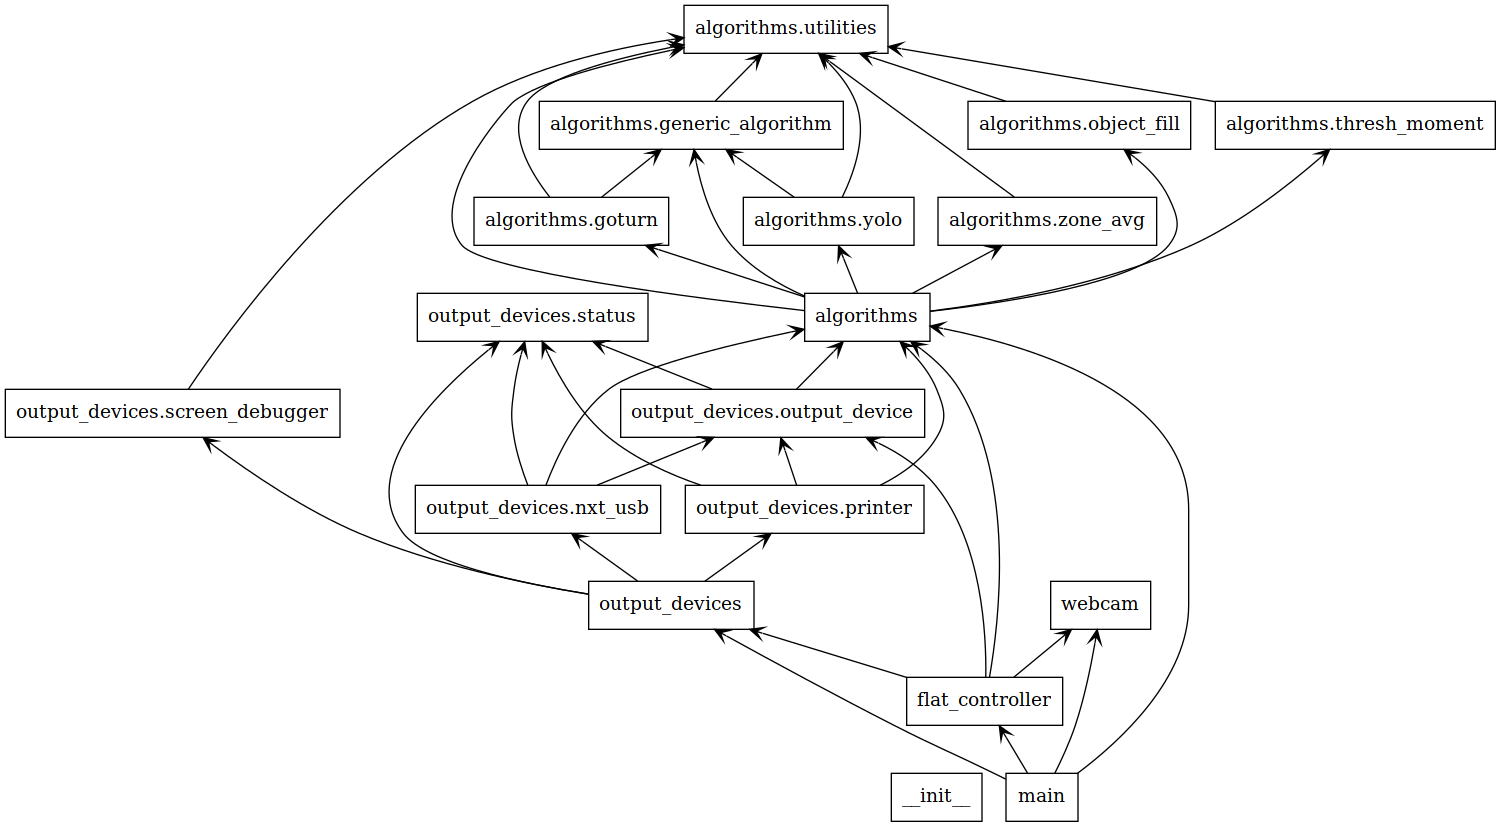
\includegraphics[width=\textwidth]{5.Solution/images/python_packages.png}
	\caption{The dependencies of the packages of the project{.} Image generated with pyreverse\cite{pyreverse}}
	\label{fig:pythonClasses}
\end{figure}


The project also contains functions for calibration, as seen on Figure~\ref{fig:pythonClasses}, which will be covered in Section~\ref{sec:calibration}.


\subsection{Movement}
The codebase of the NXT is separated into different files with distinct responsibilities, resulting in modularity, much like described above.

\begin{itemize}
	\item \texttt{tasks}
	\item \texttt{usb}
	\item \texttt{display}
	\item \texttt{movement}
	\item \texttt{calibration}
\end{itemize}

The \texttt{tasks.c} file is the entry point of the project, which creates all the tasks that should be run on the system.
\todo{Skriv om tasks.c} 
